
\section{The pseudogap vs. the coherent state}

The phase diagram for the cuprates, when hole doping is the tuning parameter, appears to be universal, however, at the time of writing, is somehwhat more complicated than that of a typical pnictide. With reference to the schematic cuprate phase diagram shown in \fig\ref{Fig:1:UniversalCupratePhaseDiagram} we see several temperature scales that may or may not be of interest to the underlying causes of \highTc superconductivity.
\begin{figure}[htbp]
    \begin{center}
        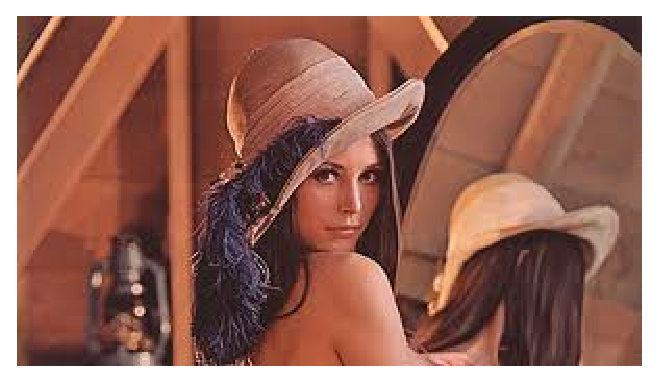
\includegraphics[scale=0.7]{Misc/TODO}
        \caption{A schematic phase diagram of a series of hole-doped cuprates}
        \label{Fig:1:UniversalCupratePhaseDiagram}
    \end{center}
\end{figure}
From the standpoint of convetional superconductivity, the first striking feature is the proximity of an antiferromagnetic phase to the superconducting region. Even without actual temperature labels, it becomes clear that if this was a phonon mediated superconductor, the pairing must be strong in order to overcome the strong spin-desnity wave scattering that results in the anitferromagnetic state.


\subsection{Anisotropic scattering}


